% ICML 2026 MI Workshop — Virtual poster
% Portrait, 24in (W) x 36in (H), within the 36x24 limit.
% Self-contained: plain article + geometry + tikz. No poster class needed.
% Build:  pdflatex poster.tex   (figures live in ../figures)
\documentclass{article}

\usepackage[paperwidth=24in,paperheight=36in,margin=1in]{geometry}
\usepackage{graphicx}
\usepackage{xcolor}
\usepackage{tikz}
\usepackage{amsmath,amssymb}
\usepackage{helvet}
\renewcommand{\familydefault}{\sfdefault}
\usepackage[T1]{fontenc}
\usepackage{booktabs}

\graphicspath{{../figures/}}

% Match the paper's shorthand for the matrix latent
\newcommand{\Z}{Z}

% ---- Theme colors -------------------------------------------------------
\definecolor{primary}{HTML}{1B3A5B}   % deep navy
\definecolor{accent}{HTML}{C9772E}    % amber
\definecolor{teal}{HTML}{1F7A6E}      % teal for "flat = blind"
\definecolor{lightbg}{HTML}{EEF2F6}   % box background
\definecolor{rule}{HTML}{9FB2C2}

\setlength{\parindent}{0pt}
\pagestyle{empty}

% ---- Font sizes for a 24x36 in poster -----------------------------------
\newcommand{\titlefont}{\fontsize{62}{70}\selectfont}
\newcommand{\subtitlefont}{\fontsize{30}{38}\selectfont}
\newcommand{\sectionfont}{\fontsize{32}{38}\selectfont\bfseries}
\newcommand{\bodyfont}{\fontsize{23}{31}\selectfont}
\newcommand{\bigfont}{\fontsize{29}{38}\selectfont}

% ---- Section header bar -------------------------------------------------
\newcommand{\sechead}[1]{%
  \vspace{6pt}%
  \colorbox{primary}{\makebox[\linewidth][l]{\rule[-6pt]{0pt}{44pt}\hspace{10pt}%
  \color{white}\sectionfont #1}}\par\vspace{7pt}}

% ---- Highlight / callout box (tikz rounded rect) ------------------------
% \callout{fill}{frame}{textcolor}{content}
\newcommand{\callout}[4]{%
  \begin{tikzpicture}
  \node[fill=#1, draw=#2, line width=3pt, rounded corners=18pt,
        inner sep=22pt, text width=\linewidth-44pt-6pt,
        align=left, text=#3] {#4};
  \end{tikzpicture}}

\begin{document}
\bodyfont

% =========================================================================
% TITLE BANNER
% =========================================================================
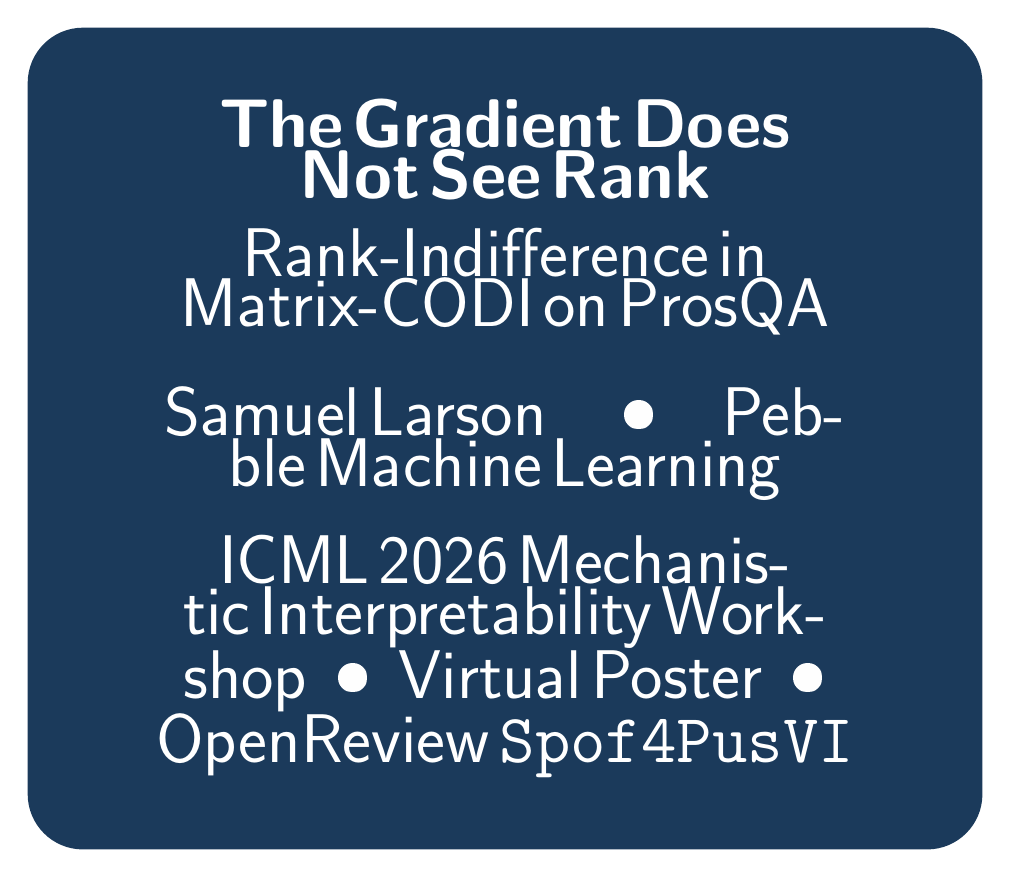
\begin{tikzpicture}
\node[fill=primary, rounded corners=20pt, inner sep=26pt,
      text width=\linewidth-52pt, align=center, text=white] {%
  {\titlefont\bfseries The Gradient Does Not See Rank}\\[10pt]
  {\subtitlefont Rank-Indifference in Matrix-CODI on ProsQA}\\[18pt]
  {\bigfont Samuel Larson \quad\textbullet\quad Pebble Machine Learning}\\[12pt]
  {\subtitlefont ICML 2026 Mechanistic Interpretability Workshop \;\textbullet\;
   Virtual Poster \;\textbullet\; OpenReview \texttt{Spof4PusVI}}%
};
\end{tikzpicture}

\vspace{8pt}

% ---- TL;DR strip --------------------------------------------------------
\callout{accent!18}{accent}{black}{%
  {\bigfont\bfseries TL;DR.\ }
  Continuous chain-of-thought stores ``parallel reasoning paths'' in the
  \emph{rank} of a matrix-valued latent $\Z$, or so the superposition
  story goes. We truncate $\Z$ to rank $k$ at inference and accuracy
  \textbf{does not move}. The training objective never rewards rank: the
  readout Jacobian carries no rank signal, four nonlinear readouts stay
  flat, and three seeds land at ranks $\{4,12,13\}$ with the same accuracy.
  The gradient is \textbf{blind to rank}.}

\vspace{8pt}

% TWO COLUMNS
% =========================================================================
\noindent
\begin{minipage}[t]{0.485\linewidth}
%% ---------- LEFT COLUMN ----------

\sechead{1.\ The setup}
\bodyfont
Matrix-CODI compresses an explicit rationale into a small number of
continuous latent positions, each a $d\times d$ matrix $\Z$:
\[
h \xrightarrow{W_{\text{up}}} \text{reshape}
  \xrightarrow{\;\text{thinker}\;} \Z
  \xrightarrow{\text{flatten}} W_{\text{down}} \to \text{answer}.
\]
$\Z$ has a computable \textbf{rank} via its SVD. \emph{If} each singular
direction encodes a separate reasoning path, truncating $\Z$ to rank $k$
should hurt accuracy once the task needs more than $k$ paths. The
\textbf{rank-$k$ ablation curve} is the natural probe.
\\[4pt]
\textit{Setup:} GPT-2 small, $d{=}16$, six latent positions, ProsQA
(also GSM8K-Aug).

\sechead{2.\ Rank-\textit{k} ablation is flat}
\begin{center}
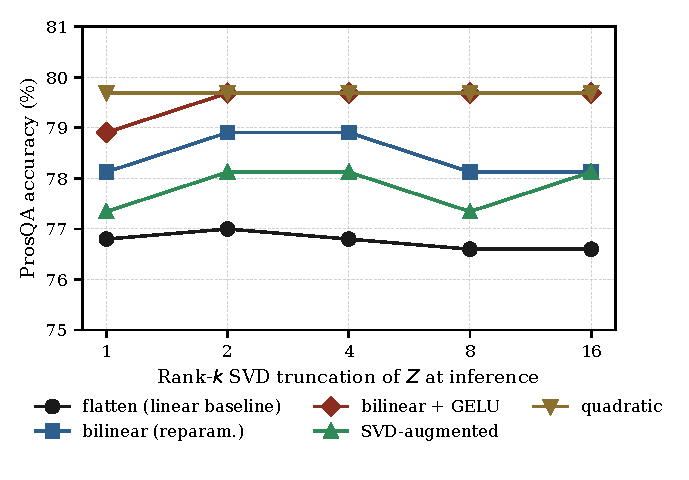
\includegraphics[width=0.66\linewidth]{fig1_rank_curves.pdf}
\end{center}
Truncating to $k\!\in\!\{1,2,4,8,16\}$ moves accuracy by
$\leq\!0.6$\,pp: flat at two distillation weights, with the
multiplicative thinker on \emph{or} off, on ProsQA \emph{and} GSM8K-Aug.
A rank-1 thought decodes as well as a full-rank one.

\sechead{3.\ Seeds decouple rank from accuracy}
\begin{center}

\includegraphics[width=0.66\linewidth]{fig2_seed_decoupling.pdf}
\end{center}
Three seeds, identical hyperparameters $\to$ effective ranks
$\{4,12,13\}$ but accuracy $81.5\pm1.2$\,pp. \textbf{Rank wanders;
accuracy doesn't.} This seed-level spread is what separates
\emph{rank-blindness} from mere position-irrelevance.

\end{minipage}\hfill
\begin{minipage}[t]{0.485\linewidth}
%% ---------- RIGHT COLUMN ----------

\sechead{4.\ Positive controls: not a flatten artifact}
\bodyfont
Maybe ``flatten then $W_{\text{down}}$'' linearizes away the rank. We test
four readouts that are \textbf{nonlinear in $\Z$} and escape the
linear-Jacobian shortcut:
\\[8pt]
\begin{center}\bigfont
\begin{tabular}{@{}ll@{}}
\toprule
\textbf{Readout} & \textbf{Spearman $p$}\\
\midrule
Bilinear              & $0.63$\\
Bilinear\,$+$\,GELU    & $0.14$\\
SVD-augmented MLP     & $0.82$\\
Quadratic $\Z\Z^\top$ & $0.46$\\
\bottomrule
\end{tabular}
\end{center}
\vspace{2pt}
All four rank-$k$ curves stay flat ($p\in[0.14,\,0.82]$). The flatness
\textbf{survives nonlinear readouts}: it is not a flatten artifact.

\sechead{5.\ The probe trap (negative control)}
\begin{center}
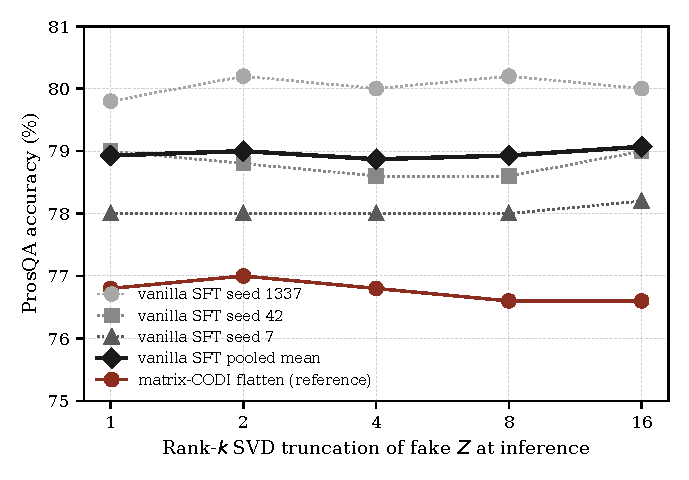
\includegraphics[width=0.66\linewidth]{fig6_negative_control.pdf}
\end{center}
Run the \emph{same} rank-$k$ intervention on vanilla GPT-2 SFT (no
matrix bottleneck, no $\Z$). It \textbf{also} produces a flat curve
(pooled range $0.20$\,pp), and a random-$h$ floor lands at the same
accuracy. \textbf{Lesson: the rank-$k$ ablation alone conflates
rank-blindness with position-irrelevance.} The seed spread (panel 3)
is the real evidence.

\sechead{6.\ The latent \textit{Z} is a weak feature}
\begin{center}
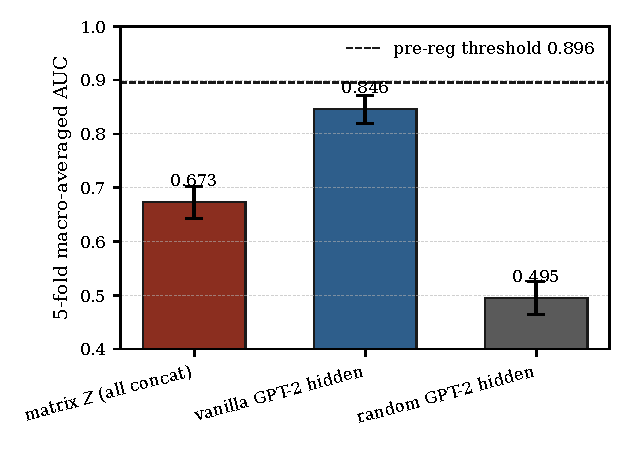
\includegraphics[width=0.66\linewidth]{fig5_linear_probe.pdf}
\end{center}
A linear probe on $\Z$ (1536 features) hits AUC $0.673$ on target
prediction; a raw pretrained GPT-2 hidden state (768 features) hits
$0.846$ on the same task. The learned matrix latent holds \emph{less}
decodable structure than the backbone it sits on.

\vspace{4pt}
\callout{teal!15}{teal}{black}{%
  {\bigfont\bfseries Takeaway.\ } CODI's objective does not reward rank:
  the Jacobian carries no rank signal, nonlinear readouts stay flat, and
  matched seeds scatter rank while pinning accuracy. ``Superposition in
  the rank'' is not learned here, and the obvious probe for it is
  itself misleading.}

\end{minipage}

% =========================================================================
% FOOTER
% =========================================================================
\vspace{10pt}
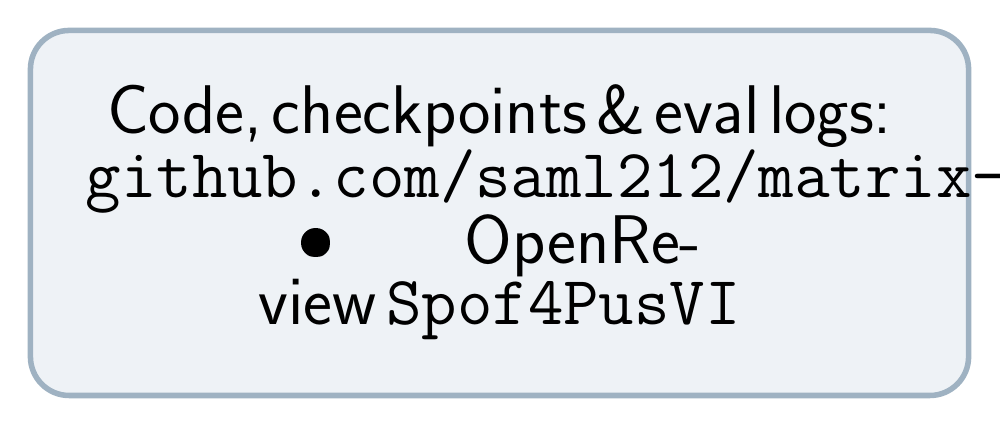
\begin{tikzpicture}
\node[fill=lightbg, draw=rule, line width=2pt, rounded corners=14pt,
      inner sep=20pt, text width=\linewidth-46pt, align=center] {%
  \bigfont Code, checkpoints \& eval logs:\;
  \texttt{github.com/saml212/matrix-codi-rank-blindness}
  \qquad\textbullet\qquad OpenReview \texttt{Spof4PusVI}};
\end{tikzpicture}

\end{document}
